\documentclass{article}

% preamble -----------------------------
% load packages 
% these are the set of packages that i typically use. we'll only discuss a few
% packages we will discuss
\usepackage{Sweave} % use sweave
\usepackage[top=.9in, bottom=.9in, left=.9in, right=.8in]{geometry} % set margins
\usepackage[pdfborder={0 0 0}]{hyperref}% For email addresses
  \hypersetup{ % make TOC clickable links
    colorlinks,
    citecolor=black,
    filecolor=black,
    linkcolor=blue,
    urlcolor=black
  }
\usepackage[draft]{fixme} % enable comments in the margins
  \fxsetup{layout=footnote, marginclue}
\usepackage{lineno,xcolor}% Running line numbers:
  \linenumbers
  \setlength\linenumbersep{5pt}
  \renewcommand\linenumberfont{\normalfont\tiny\sffamily\color{gray}}

% packages we won't discuss
\usepackage{fullpage}
\usepackage{float} 
\usepackage{enumerate}
\usepackage[utf8]{inputenc}
\usepackage{titling}
\usepackage{caption}
\usepackage{subcaption}
\setlength{\droptitle}{-4em} 
\usepackage{amsmath}
\usepackage{natbib} % unnumbered bibliography style
\usepackage{indentfirst} % indent first paragraph of a section
\usepackage{chngcntr} % for appendix figure counting
\usepackage{authblk}


% preamble ----------------------------


\begin{document}
\Sconcordance{concordance:Demo_Cory.tex:Demo_Cory.Rnw:%
1 70 1 1 3 2 0 2 1 4 0 1 2 1 3 2 0 3 1 8 0 1 2 1 3 2 0 3 1 3 0 1 2 1 3 %
2 0 4 1 4 0 1 2 1 7 6 0 1 2 1 5 1 2 1 4 19 0 1 2 8 1}


\title{practice doc}
\author{Cory}
\maketitle
\tableofcontents

\section*{Abstract}

jdgkjbsdfhjkgbkdbvjklnvz dfk.jbnv.jdbjdfnzk. jbvnfjdfjznbj;dnfz gbjnfljnbjdzn bfj;dzojfbnojdznf bkjndzfjbnkzdjfn bkjzbnzjdnfbljkzdnfbjlknzdl jfbnnodznbgondzounos;nzdjbnfkjdnzk;bn;odz b;ohb;ohzdo;bhz;bdh fodhobhozdb hflzdnf. \fxnote{this paragraph is awful}

% here's a note

\section{Introduction}

\textbf{context for the paper}

\begin{itemize}
  \item point 1
  \item point 2
\end{itemize}

\begin{enumerate}
  \item point 1 
\end{enumerate}

\section{Results}

\begin{Schunk}
\begin{Sinput}
> #chunk 1
> x=rnorm(10)
> y=rnorm(10)
> plot(x,y)
\end{Sinput}
\end{Schunk}
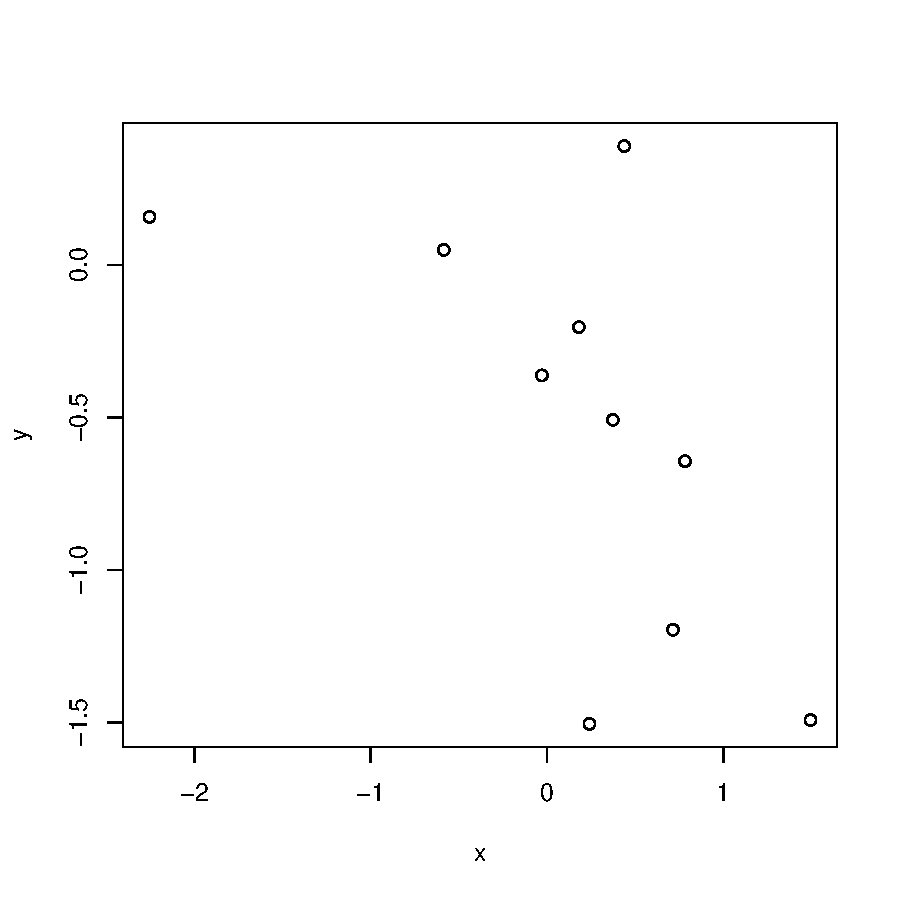
\includegraphics{Demo_Cory-chunk_name}

\begin{Schunk}
\begin{Sinput}
> #chunk 2
> x=rnorm(10)
> y=rnorm(10)
> plot(x,y)
> print(x)
\end{Sinput}
\begin{Soutput}
 [1] -2.0928386 -0.2465789  1.2137872  1.7635851 -1.9904315  2.4824153
 [7] -2.7284000  1.6391409  1.0957504  0.7413645
\end{Soutput}
\end{Schunk}
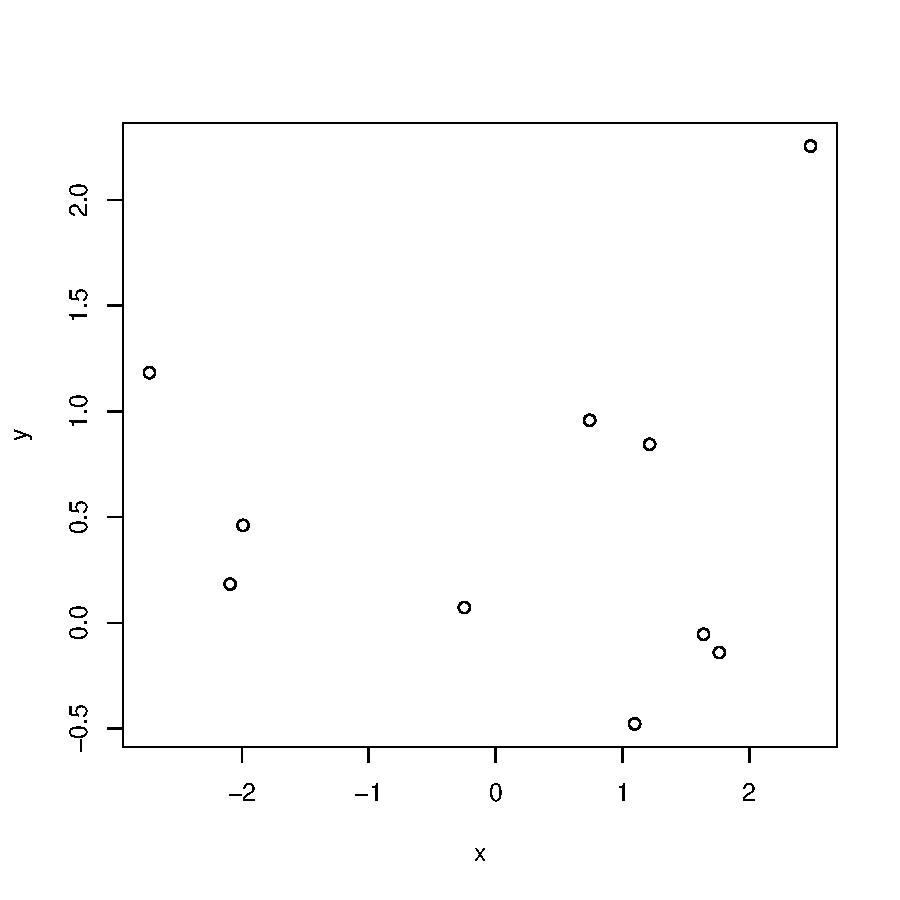
\includegraphics{Demo_Cory-chunk_name1_5}

\begin{Schunk}
\begin{Sinput}
> #chunk 3
> x=rnorm(10)
> y=rnorm(10)
> z=rnorm(10)
> plot(x,y)
\end{Sinput}
\end{Schunk}

\begin{Schunk}
\begin{Sinput}
> #chunk 4 - results=hide
> x=rnorm(10)
> y=rnorm(10)
> z=rnorm(10)
> plot(x,y)
> print(x)
\end{Sinput}
\end{Schunk}
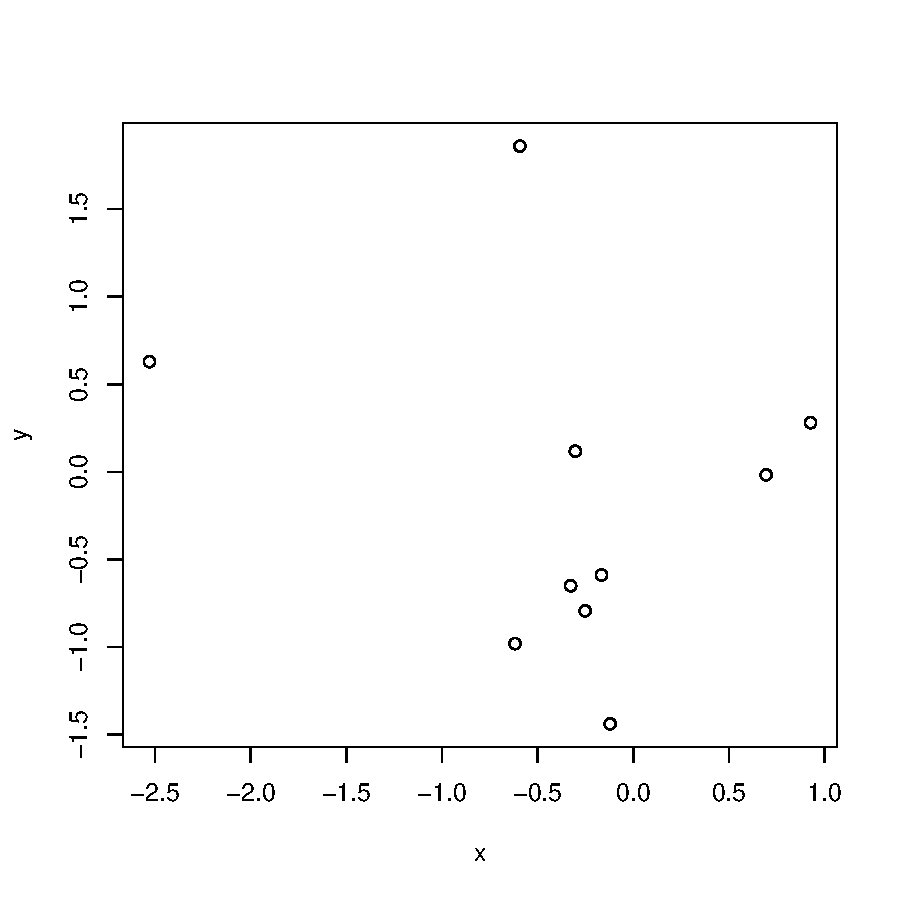
\includegraphics{Demo_Cory-chunk_name4}

\begin{Schunk}
\begin{Soutput}
 [1] -0.4930552 -0.4433611 -0.4831262  1.8740668 -0.1244868  0.6099862
 [7] -0.3598758 -1.9720957 -0.3541495  0.2759110
\end{Soutput}
\end{Schunk}
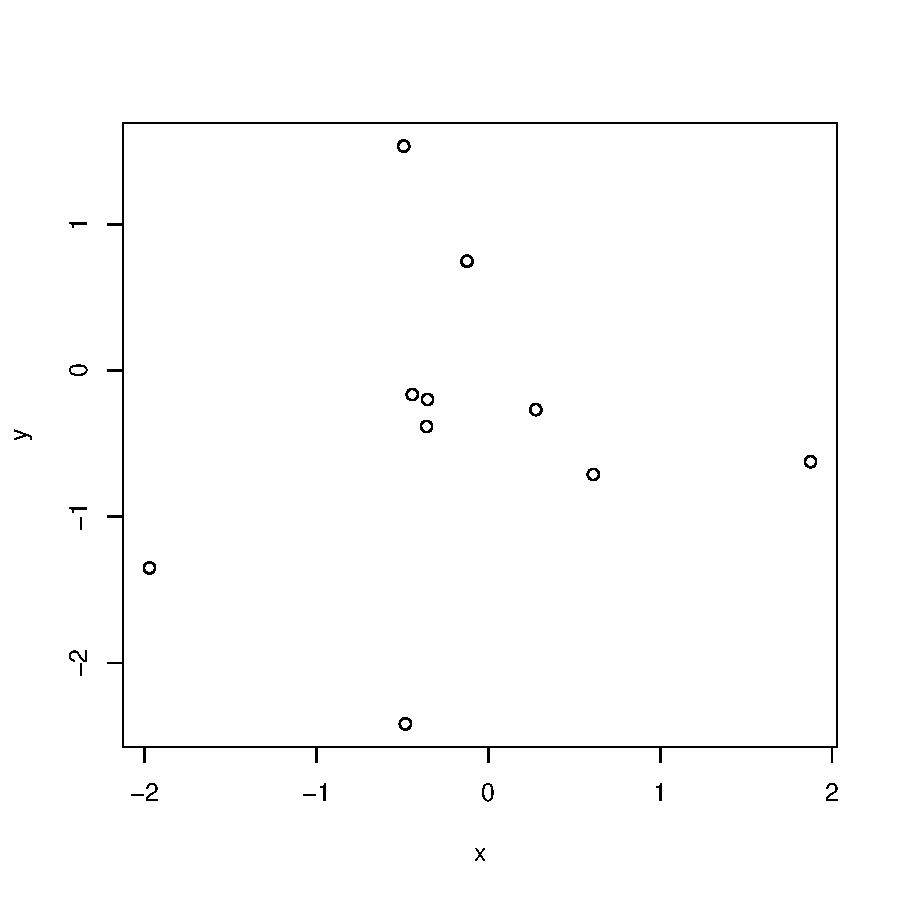
\includegraphics{Demo_Cory-chunk_name5}

\includegraphics{Demo_Cory-chunk_name6}

% latex table generated in R 3.2.2 by xtable 1.8-0 package
% Tue Jan 26 14:52:31 2016
\begin{table}[ht]
\centering
\begin{tabular}{rrr}
  \hline
 & x & y \\ 
  \hline
1 & 0.35 & 0.15 \\ 
  2 & 0.57 & -0.07 \\ 
  3 & -0.13 & -0.20 \\ 
  4 & 0.45 & 0.21 \\ 
  5 & 0.37 & -0.20 \\ 
  6 & 1.49 & -2.07 \\ 
  7 & -0.97 & 0.64 \\ 
  8 & -0.81 & -1.40 \\ 
  9 & 0.60 & 0.04 \\ 
  10 & -1.18 & -0.58 \\ 
   \hline
\end{tabular}
\end{table}







\end{document}
